\documentclass[11pt]{article}

    \usepackage[breakable]{tcolorbox}
    \usepackage{parskip} % Stop auto-indenting (to mimic markdown behaviour)
    

    % Basic figure setup, for now with no caption control since it's done
    % automatically by Pandoc (which extracts ![](path) syntax from Markdown).
    \usepackage{graphicx}
    % Keep aspect ratio if custom image width or height is specified
    \setkeys{Gin}{keepaspectratio}
    % Maintain compatibility with old templates. Remove in nbconvert 6.0
    \let\Oldincludegraphics\includegraphics
    % Ensure that by default, figures have no caption (until we provide a
    % proper Figure object with a Caption API and a way to capture that
    % in the conversion process - todo).
    \usepackage{caption}
    \DeclareCaptionFormat{nocaption}{}
    \captionsetup{format=nocaption,aboveskip=0pt,belowskip=0pt}

    \usepackage{float}
    \floatplacement{figure}{H} % forces figures to be placed at the correct location
    \usepackage{xcolor} % Allow colors to be defined
    \usepackage{enumerate} % Needed for markdown enumerations to work
    \usepackage{geometry} % Used to adjust the document margins
    \usepackage{amsmath} % Equations
    \usepackage{amssymb} % Equations
    \usepackage{textcomp} % defines textquotesingle
    % Hack from http://tex.stackexchange.com/a/47451/13684:
    \AtBeginDocument{%
        \def\PYZsq{\textquotesingle}% Upright quotes in Pygmentized code
    }
    \usepackage{upquote} % Upright quotes for verbatim code
    \usepackage{eurosym} % defines \euro

    \usepackage{iftex}
    \ifPDFTeX
        \usepackage[T1]{fontenc}
        \IfFileExists{alphabeta.sty}{
              \usepackage{alphabeta}
          }{
              \usepackage[mathletters]{ucs}
              \usepackage[utf8x]{inputenc}
          }
    \else
        \usepackage{fontspec}
        \usepackage{unicode-math}
    \fi

    \usepackage{fancyvrb} % verbatim replacement that allows latex
    \usepackage{grffile} % extends the file name processing of package graphics
                         % to support a larger range
    \makeatletter % fix for old versions of grffile with XeLaTeX
    \@ifpackagelater{grffile}{2019/11/01}
    {
      % Do nothing on new versions
    }
    {
      \def\Gread@@xetex#1{%
        \IfFileExists{"\Gin@base".bb}%
        {\Gread@eps{\Gin@base.bb}}%
        {\Gread@@xetex@aux#1}%
      }
    }
    \makeatother
    \usepackage[Export]{adjustbox} % Used to constrain images to a maximum size
    \adjustboxset{max size={0.9\linewidth}{0.9\paperheight}}

    % The hyperref package gives us a pdf with properly built
    % internal navigation ('pdf bookmarks' for the table of contents,
    % internal cross-reference links, web links for URLs, etc.)
    \usepackage{hyperref}
    % The default LaTeX title has an obnoxious amount of whitespace. By default,
    % titling removes some of it. It also provides customization options.
    \usepackage{titling}
    \usepackage{longtable} % longtable support required by pandoc >1.10
    \usepackage{booktabs}  % table support for pandoc > 1.12.2
    \usepackage{array}     % table support for pandoc >= 2.11.3
    \usepackage{calc}      % table minipage width calculation for pandoc >= 2.11.1
    \usepackage[inline]{enumitem} % IRkernel/repr support (it uses the enumerate* environment)
    \usepackage[normalem]{ulem} % ulem is needed to support strikethroughs (\sout)
                                % normalem makes italics be italics, not underlines
    \usepackage{soul}      % strikethrough (\st) support for pandoc >= 3.0.0
    \usepackage{mathrsfs}
    

    
    % Colors for the hyperref package
    \definecolor{urlcolor}{rgb}{0,.145,.698}
    \definecolor{linkcolor}{rgb}{.71,0.21,0.01}
    \definecolor{citecolor}{rgb}{.12,.54,.11}

    % ANSI colors
    \definecolor{ansi-black}{HTML}{3E424D}
    \definecolor{ansi-black-intense}{HTML}{282C36}
    \definecolor{ansi-red}{HTML}{E75C58}
    \definecolor{ansi-red-intense}{HTML}{B22B31}
    \definecolor{ansi-green}{HTML}{00A250}
    \definecolor{ansi-green-intense}{HTML}{007427}
    \definecolor{ansi-yellow}{HTML}{DDB62B}
    \definecolor{ansi-yellow-intense}{HTML}{B27D12}
    \definecolor{ansi-blue}{HTML}{208FFB}
    \definecolor{ansi-blue-intense}{HTML}{0065CA}
    \definecolor{ansi-magenta}{HTML}{D160C4}
    \definecolor{ansi-magenta-intense}{HTML}{A03196}
    \definecolor{ansi-cyan}{HTML}{60C6C8}
    \definecolor{ansi-cyan-intense}{HTML}{258F8F}
    \definecolor{ansi-white}{HTML}{C5C1B4}
    \definecolor{ansi-white-intense}{HTML}{A1A6B2}
    \definecolor{ansi-default-inverse-fg}{HTML}{FFFFFF}
    \definecolor{ansi-default-inverse-bg}{HTML}{000000}

    % common color for the border for error outputs.
    \definecolor{outerrorbackground}{HTML}{FFDFDF}

    % commands and environments needed by pandoc snippets
    % extracted from the output of `pandoc -s`
    \providecommand{\tightlist}{%
      \setlength{\itemsep}{0pt}\setlength{\parskip}{0pt}}
    \DefineVerbatimEnvironment{Highlighting}{Verbatim}{commandchars=\\\{\}}
    % Add ',fontsize=\small' for more characters per line
    \newenvironment{Shaded}{}{}
    \newcommand{\KeywordTok}[1]{\textcolor[rgb]{0.00,0.44,0.13}{\textbf{{#1}}}}
    \newcommand{\DataTypeTok}[1]{\textcolor[rgb]{0.56,0.13,0.00}{{#1}}}
    \newcommand{\DecValTok}[1]{\textcolor[rgb]{0.25,0.63,0.44}{{#1}}}
    \newcommand{\BaseNTok}[1]{\textcolor[rgb]{0.25,0.63,0.44}{{#1}}}
    \newcommand{\FloatTok}[1]{\textcolor[rgb]{0.25,0.63,0.44}{{#1}}}
    \newcommand{\CharTok}[1]{\textcolor[rgb]{0.25,0.44,0.63}{{#1}}}
    \newcommand{\StringTok}[1]{\textcolor[rgb]{0.25,0.44,0.63}{{#1}}}
    \newcommand{\CommentTok}[1]{\textcolor[rgb]{0.38,0.63,0.69}{\textit{{#1}}}}
    \newcommand{\OtherTok}[1]{\textcolor[rgb]{0.00,0.44,0.13}{{#1}}}
    \newcommand{\AlertTok}[1]{\textcolor[rgb]{1.00,0.00,0.00}{\textbf{{#1}}}}
    \newcommand{\FunctionTok}[1]{\textcolor[rgb]{0.02,0.16,0.49}{{#1}}}
    \newcommand{\RegionMarkerTok}[1]{{#1}}
    \newcommand{\ErrorTok}[1]{\textcolor[rgb]{1.00,0.00,0.00}{\textbf{{#1}}}}
    \newcommand{\NormalTok}[1]{{#1}}

    % Additional commands for more recent versions of Pandoc
    \newcommand{\ConstantTok}[1]{\textcolor[rgb]{0.53,0.00,0.00}{{#1}}}
    \newcommand{\SpecialCharTok}[1]{\textcolor[rgb]{0.25,0.44,0.63}{{#1}}}
    \newcommand{\VerbatimStringTok}[1]{\textcolor[rgb]{0.25,0.44,0.63}{{#1}}}
    \newcommand{\SpecialStringTok}[1]{\textcolor[rgb]{0.73,0.40,0.53}{{#1}}}
    \newcommand{\ImportTok}[1]{{#1}}
    \newcommand{\DocumentationTok}[1]{\textcolor[rgb]{0.73,0.13,0.13}{\textit{{#1}}}}
    \newcommand{\AnnotationTok}[1]{\textcolor[rgb]{0.38,0.63,0.69}{\textbf{\textit{{#1}}}}}
    \newcommand{\CommentVarTok}[1]{\textcolor[rgb]{0.38,0.63,0.69}{\textbf{\textit{{#1}}}}}
    \newcommand{\VariableTok}[1]{\textcolor[rgb]{0.10,0.09,0.49}{{#1}}}
    \newcommand{\ControlFlowTok}[1]{\textcolor[rgb]{0.00,0.44,0.13}{\textbf{{#1}}}}
    \newcommand{\OperatorTok}[1]{\textcolor[rgb]{0.40,0.40,0.40}{{#1}}}
    \newcommand{\BuiltInTok}[1]{{#1}}
    \newcommand{\ExtensionTok}[1]{{#1}}
    \newcommand{\PreprocessorTok}[1]{\textcolor[rgb]{0.74,0.48,0.00}{{#1}}}
    \newcommand{\AttributeTok}[1]{\textcolor[rgb]{0.49,0.56,0.16}{{#1}}}
    \newcommand{\InformationTok}[1]{\textcolor[rgb]{0.38,0.63,0.69}{\textbf{\textit{{#1}}}}}
    \newcommand{\WarningTok}[1]{\textcolor[rgb]{0.38,0.63,0.69}{\textbf{\textit{{#1}}}}}


    % Define a nice break command that doesn't care if a line doesn't already
    % exist.
    \def\br{\hspace*{\fill} \\* }
    % Math Jax compatibility definitions
    \def\gt{>}
    \def\lt{<}
    \let\Oldtex\TeX
    \let\Oldlatex\LaTeX
    \renewcommand{\TeX}{\textrm{\Oldtex}}
    \renewcommand{\LaTeX}{\textrm{\Oldlatex}}
    % Document parameters
    % Document title
    \title{MathEng2223}
    
    
    
    
    
    
    
% Pygments definitions
\makeatletter
\def\PY@reset{\let\PY@it=\relax \let\PY@bf=\relax%
    \let\PY@ul=\relax \let\PY@tc=\relax%
    \let\PY@bc=\relax \let\PY@ff=\relax}
\def\PY@tok#1{\csname PY@tok@#1\endcsname}
\def\PY@toks#1+{\ifx\relax#1\empty\else%
    \PY@tok{#1}\expandafter\PY@toks\fi}
\def\PY@do#1{\PY@bc{\PY@tc{\PY@ul{%
    \PY@it{\PY@bf{\PY@ff{#1}}}}}}}
\def\PY#1#2{\PY@reset\PY@toks#1+\relax+\PY@do{#2}}

\@namedef{PY@tok@w}{\def\PY@tc##1{\textcolor[rgb]{0.73,0.73,0.73}{##1}}}
\@namedef{PY@tok@c}{\let\PY@it=\textit\def\PY@tc##1{\textcolor[rgb]{0.24,0.48,0.48}{##1}}}
\@namedef{PY@tok@cp}{\def\PY@tc##1{\textcolor[rgb]{0.61,0.40,0.00}{##1}}}
\@namedef{PY@tok@k}{\let\PY@bf=\textbf\def\PY@tc##1{\textcolor[rgb]{0.00,0.50,0.00}{##1}}}
\@namedef{PY@tok@kp}{\def\PY@tc##1{\textcolor[rgb]{0.00,0.50,0.00}{##1}}}
\@namedef{PY@tok@kt}{\def\PY@tc##1{\textcolor[rgb]{0.69,0.00,0.25}{##1}}}
\@namedef{PY@tok@o}{\def\PY@tc##1{\textcolor[rgb]{0.40,0.40,0.40}{##1}}}
\@namedef{PY@tok@ow}{\let\PY@bf=\textbf\def\PY@tc##1{\textcolor[rgb]{0.67,0.13,1.00}{##1}}}
\@namedef{PY@tok@nb}{\def\PY@tc##1{\textcolor[rgb]{0.00,0.50,0.00}{##1}}}
\@namedef{PY@tok@nf}{\def\PY@tc##1{\textcolor[rgb]{0.00,0.00,1.00}{##1}}}
\@namedef{PY@tok@nc}{\let\PY@bf=\textbf\def\PY@tc##1{\textcolor[rgb]{0.00,0.00,1.00}{##1}}}
\@namedef{PY@tok@nn}{\let\PY@bf=\textbf\def\PY@tc##1{\textcolor[rgb]{0.00,0.00,1.00}{##1}}}
\@namedef{PY@tok@ne}{\let\PY@bf=\textbf\def\PY@tc##1{\textcolor[rgb]{0.80,0.25,0.22}{##1}}}
\@namedef{PY@tok@nv}{\def\PY@tc##1{\textcolor[rgb]{0.10,0.09,0.49}{##1}}}
\@namedef{PY@tok@no}{\def\PY@tc##1{\textcolor[rgb]{0.53,0.00,0.00}{##1}}}
\@namedef{PY@tok@nl}{\def\PY@tc##1{\textcolor[rgb]{0.46,0.46,0.00}{##1}}}
\@namedef{PY@tok@ni}{\let\PY@bf=\textbf\def\PY@tc##1{\textcolor[rgb]{0.44,0.44,0.44}{##1}}}
\@namedef{PY@tok@na}{\def\PY@tc##1{\textcolor[rgb]{0.41,0.47,0.13}{##1}}}
\@namedef{PY@tok@nt}{\let\PY@bf=\textbf\def\PY@tc##1{\textcolor[rgb]{0.00,0.50,0.00}{##1}}}
\@namedef{PY@tok@nd}{\def\PY@tc##1{\textcolor[rgb]{0.67,0.13,1.00}{##1}}}
\@namedef{PY@tok@s}{\def\PY@tc##1{\textcolor[rgb]{0.73,0.13,0.13}{##1}}}
\@namedef{PY@tok@sd}{\let\PY@it=\textit\def\PY@tc##1{\textcolor[rgb]{0.73,0.13,0.13}{##1}}}
\@namedef{PY@tok@si}{\let\PY@bf=\textbf\def\PY@tc##1{\textcolor[rgb]{0.64,0.35,0.47}{##1}}}
\@namedef{PY@tok@se}{\let\PY@bf=\textbf\def\PY@tc##1{\textcolor[rgb]{0.67,0.36,0.12}{##1}}}
\@namedef{PY@tok@sr}{\def\PY@tc##1{\textcolor[rgb]{0.64,0.35,0.47}{##1}}}
\@namedef{PY@tok@ss}{\def\PY@tc##1{\textcolor[rgb]{0.10,0.09,0.49}{##1}}}
\@namedef{PY@tok@sx}{\def\PY@tc##1{\textcolor[rgb]{0.00,0.50,0.00}{##1}}}
\@namedef{PY@tok@m}{\def\PY@tc##1{\textcolor[rgb]{0.40,0.40,0.40}{##1}}}
\@namedef{PY@tok@gh}{\let\PY@bf=\textbf\def\PY@tc##1{\textcolor[rgb]{0.00,0.00,0.50}{##1}}}
\@namedef{PY@tok@gu}{\let\PY@bf=\textbf\def\PY@tc##1{\textcolor[rgb]{0.50,0.00,0.50}{##1}}}
\@namedef{PY@tok@gd}{\def\PY@tc##1{\textcolor[rgb]{0.63,0.00,0.00}{##1}}}
\@namedef{PY@tok@gi}{\def\PY@tc##1{\textcolor[rgb]{0.00,0.52,0.00}{##1}}}
\@namedef{PY@tok@gr}{\def\PY@tc##1{\textcolor[rgb]{0.89,0.00,0.00}{##1}}}
\@namedef{PY@tok@ge}{\let\PY@it=\textit}
\@namedef{PY@tok@gs}{\let\PY@bf=\textbf}
\@namedef{PY@tok@ges}{\let\PY@bf=\textbf\let\PY@it=\textit}
\@namedef{PY@tok@gp}{\let\PY@bf=\textbf\def\PY@tc##1{\textcolor[rgb]{0.00,0.00,0.50}{##1}}}
\@namedef{PY@tok@go}{\def\PY@tc##1{\textcolor[rgb]{0.44,0.44,0.44}{##1}}}
\@namedef{PY@tok@gt}{\def\PY@tc##1{\textcolor[rgb]{0.00,0.27,0.87}{##1}}}
\@namedef{PY@tok@err}{\def\PY@bc##1{{\setlength{\fboxsep}{\string -\fboxrule}\fcolorbox[rgb]{1.00,0.00,0.00}{1,1,1}{\strut ##1}}}}
\@namedef{PY@tok@kc}{\let\PY@bf=\textbf\def\PY@tc##1{\textcolor[rgb]{0.00,0.50,0.00}{##1}}}
\@namedef{PY@tok@kd}{\let\PY@bf=\textbf\def\PY@tc##1{\textcolor[rgb]{0.00,0.50,0.00}{##1}}}
\@namedef{PY@tok@kn}{\let\PY@bf=\textbf\def\PY@tc##1{\textcolor[rgb]{0.00,0.50,0.00}{##1}}}
\@namedef{PY@tok@kr}{\let\PY@bf=\textbf\def\PY@tc##1{\textcolor[rgb]{0.00,0.50,0.00}{##1}}}
\@namedef{PY@tok@bp}{\def\PY@tc##1{\textcolor[rgb]{0.00,0.50,0.00}{##1}}}
\@namedef{PY@tok@fm}{\def\PY@tc##1{\textcolor[rgb]{0.00,0.00,1.00}{##1}}}
\@namedef{PY@tok@vc}{\def\PY@tc##1{\textcolor[rgb]{0.10,0.09,0.49}{##1}}}
\@namedef{PY@tok@vg}{\def\PY@tc##1{\textcolor[rgb]{0.10,0.09,0.49}{##1}}}
\@namedef{PY@tok@vi}{\def\PY@tc##1{\textcolor[rgb]{0.10,0.09,0.49}{##1}}}
\@namedef{PY@tok@vm}{\def\PY@tc##1{\textcolor[rgb]{0.10,0.09,0.49}{##1}}}
\@namedef{PY@tok@sa}{\def\PY@tc##1{\textcolor[rgb]{0.73,0.13,0.13}{##1}}}
\@namedef{PY@tok@sb}{\def\PY@tc##1{\textcolor[rgb]{0.73,0.13,0.13}{##1}}}
\@namedef{PY@tok@sc}{\def\PY@tc##1{\textcolor[rgb]{0.73,0.13,0.13}{##1}}}
\@namedef{PY@tok@dl}{\def\PY@tc##1{\textcolor[rgb]{0.73,0.13,0.13}{##1}}}
\@namedef{PY@tok@s2}{\def\PY@tc##1{\textcolor[rgb]{0.73,0.13,0.13}{##1}}}
\@namedef{PY@tok@sh}{\def\PY@tc##1{\textcolor[rgb]{0.73,0.13,0.13}{##1}}}
\@namedef{PY@tok@s1}{\def\PY@tc##1{\textcolor[rgb]{0.73,0.13,0.13}{##1}}}
\@namedef{PY@tok@mb}{\def\PY@tc##1{\textcolor[rgb]{0.40,0.40,0.40}{##1}}}
\@namedef{PY@tok@mf}{\def\PY@tc##1{\textcolor[rgb]{0.40,0.40,0.40}{##1}}}
\@namedef{PY@tok@mh}{\def\PY@tc##1{\textcolor[rgb]{0.40,0.40,0.40}{##1}}}
\@namedef{PY@tok@mi}{\def\PY@tc##1{\textcolor[rgb]{0.40,0.40,0.40}{##1}}}
\@namedef{PY@tok@il}{\def\PY@tc##1{\textcolor[rgb]{0.40,0.40,0.40}{##1}}}
\@namedef{PY@tok@mo}{\def\PY@tc##1{\textcolor[rgb]{0.40,0.40,0.40}{##1}}}
\@namedef{PY@tok@ch}{\let\PY@it=\textit\def\PY@tc##1{\textcolor[rgb]{0.24,0.48,0.48}{##1}}}
\@namedef{PY@tok@cm}{\let\PY@it=\textit\def\PY@tc##1{\textcolor[rgb]{0.24,0.48,0.48}{##1}}}
\@namedef{PY@tok@cpf}{\let\PY@it=\textit\def\PY@tc##1{\textcolor[rgb]{0.24,0.48,0.48}{##1}}}
\@namedef{PY@tok@c1}{\let\PY@it=\textit\def\PY@tc##1{\textcolor[rgb]{0.24,0.48,0.48}{##1}}}
\@namedef{PY@tok@cs}{\let\PY@it=\textit\def\PY@tc##1{\textcolor[rgb]{0.24,0.48,0.48}{##1}}}

\def\PYZbs{\char`\\}
\def\PYZus{\char`\_}
\def\PYZob{\char`\{}
\def\PYZcb{\char`\}}
\def\PYZca{\char`\^}
\def\PYZam{\char`\&}
\def\PYZlt{\char`\<}
\def\PYZgt{\char`\>}
\def\PYZsh{\char`\#}
\def\PYZpc{\char`\%}
\def\PYZdl{\char`\$}
\def\PYZhy{\char`\-}
\def\PYZsq{\char`\'}
\def\PYZdq{\char`\"}
\def\PYZti{\char`\~}
% for compatibility with earlier versions
\def\PYZat{@}
\def\PYZlb{[}
\def\PYZrb{]}
\makeatother


    % For linebreaks inside Verbatim environment from package fancyvrb.
    \makeatletter
        \newbox\Wrappedcontinuationbox
        \newbox\Wrappedvisiblespacebox
        \newcommand*\Wrappedvisiblespace {\textcolor{red}{\textvisiblespace}}
        \newcommand*\Wrappedcontinuationsymbol {\textcolor{red}{\llap{\tiny$\m@th\hookrightarrow$}}}
        \newcommand*\Wrappedcontinuationindent {3ex }
        \newcommand*\Wrappedafterbreak {\kern\Wrappedcontinuationindent\copy\Wrappedcontinuationbox}
        % Take advantage of the already applied Pygments mark-up to insert
        % potential linebreaks for TeX processing.
        %        {, <, #, %, $, ' and ": go to next line.
        %        _, }, ^, &, >, - and ~: stay at end of broken line.
        % Use of \textquotesingle for straight quote.
        \newcommand*\Wrappedbreaksatspecials {%
            \def\PYGZus{\discretionary{\char`\_}{\Wrappedafterbreak}{\char`\_}}%
            \def\PYGZob{\discretionary{}{\Wrappedafterbreak\char`\{}{\char`\{}}%
            \def\PYGZcb{\discretionary{\char`\}}{\Wrappedafterbreak}{\char`\}}}%
            \def\PYGZca{\discretionary{\char`\^}{\Wrappedafterbreak}{\char`\^}}%
            \def\PYGZam{\discretionary{\char`\&}{\Wrappedafterbreak}{\char`\&}}%
            \def\PYGZlt{\discretionary{}{\Wrappedafterbreak\char`\<}{\char`\<}}%
            \def\PYGZgt{\discretionary{\char`\>}{\Wrappedafterbreak}{\char`\>}}%
            \def\PYGZsh{\discretionary{}{\Wrappedafterbreak\char`\#}{\char`\#}}%
            \def\PYGZpc{\discretionary{}{\Wrappedafterbreak\char`\%}{\char`\%}}%
            \def\PYGZdl{\discretionary{}{\Wrappedafterbreak\char`\$}{\char`\$}}%
            \def\PYGZhy{\discretionary{\char`\-}{\Wrappedafterbreak}{\char`\-}}%
            \def\PYGZsq{\discretionary{}{\Wrappedafterbreak\textquotesingle}{\textquotesingle}}%
            \def\PYGZdq{\discretionary{}{\Wrappedafterbreak\char`\"}{\char`\"}}%
            \def\PYGZti{\discretionary{\char`\~}{\Wrappedafterbreak}{\char`\~}}%
        }
        % Some characters . , ; ? ! / are not pygmentized.
        % This macro makes them "active" and they will insert potential linebreaks
        \newcommand*\Wrappedbreaksatpunct {%
            \lccode`\~`\.\lowercase{\def~}{\discretionary{\hbox{\char`\.}}{\Wrappedafterbreak}{\hbox{\char`\.}}}%
            \lccode`\~`\,\lowercase{\def~}{\discretionary{\hbox{\char`\,}}{\Wrappedafterbreak}{\hbox{\char`\,}}}%
            \lccode`\~`\;\lowercase{\def~}{\discretionary{\hbox{\char`\;}}{\Wrappedafterbreak}{\hbox{\char`\;}}}%
            \lccode`\~`\:\lowercase{\def~}{\discretionary{\hbox{\char`\:}}{\Wrappedafterbreak}{\hbox{\char`\:}}}%
            \lccode`\~`\?\lowercase{\def~}{\discretionary{\hbox{\char`\?}}{\Wrappedafterbreak}{\hbox{\char`\?}}}%
            \lccode`\~`\!\lowercase{\def~}{\discretionary{\hbox{\char`\!}}{\Wrappedafterbreak}{\hbox{\char`\!}}}%
            \lccode`\~`\/\lowercase{\def~}{\discretionary{\hbox{\char`\/}}{\Wrappedafterbreak}{\hbox{\char`\/}}}%
            \catcode`\.\active
            \catcode`\,\active
            \catcode`\;\active
            \catcode`\:\active
            \catcode`\?\active
            \catcode`\!\active
            \catcode`\/\active
            \lccode`\~`\~
        }
    \makeatother

    \let\OriginalVerbatim=\Verbatim
    \makeatletter
    \renewcommand{\Verbatim}[1][1]{%
        %\parskip\z@skip
        \sbox\Wrappedcontinuationbox {\Wrappedcontinuationsymbol}%
        \sbox\Wrappedvisiblespacebox {\FV@SetupFont\Wrappedvisiblespace}%
        \def\FancyVerbFormatLine ##1{\hsize\linewidth
            \vtop{\raggedright\hyphenpenalty\z@\exhyphenpenalty\z@
                \doublehyphendemerits\z@\finalhyphendemerits\z@
                \strut ##1\strut}%
        }%
        % If the linebreak is at a space, the latter will be displayed as visible
        % space at end of first line, and a continuation symbol starts next line.
        % Stretch/shrink are however usually zero for typewriter font.
        \def\FV@Space {%
            \nobreak\hskip\z@ plus\fontdimen3\font minus\fontdimen4\font
            \discretionary{\copy\Wrappedvisiblespacebox}{\Wrappedafterbreak}
            {\kern\fontdimen2\font}%
        }%

        % Allow breaks at special characters using \PYG... macros.
        \Wrappedbreaksatspecials
        % Breaks at punctuation characters . , ; ? ! and / need catcode=\active
        \OriginalVerbatim[#1,codes*=\Wrappedbreaksatpunct]%
    }
    \makeatother

    % Exact colors from NB
    \definecolor{incolor}{HTML}{303F9F}
    \definecolor{outcolor}{HTML}{D84315}
    \definecolor{cellborder}{HTML}{CFCFCF}
    \definecolor{cellbackground}{HTML}{F7F7F7}

    % prompt
    \makeatletter
    \newcommand{\boxspacing}{\kern\kvtcb@left@rule\kern\kvtcb@boxsep}
    \makeatother
    \newcommand{\prompt}[4]{
        {\ttfamily\llap{{\color{#2}[#3]:\hspace{3pt}#4}}\vspace{-\baselineskip}}
    }
    

    
    % Prevent overflowing lines due to hard-to-break entities
    \sloppy
    % Setup hyperref package
    \hypersetup{
      breaklinks=true,  % so long urls are correctly broken across lines
      colorlinks=true,
      urlcolor=urlcolor,
      linkcolor=linkcolor,
      citecolor=citecolor,
      }
    % Slightly bigger margins than the latex defaults
    
    \geometry{verbose,tmargin=1in,bmargin=1in,lmargin=1in,rmargin=1in}
    
    

\begin{document}
    
    \maketitle
    
    

    
    \textbf{\emph{Mathematical Methods for Engineers (MathEng)}}

\textbf{EXAM}

\textbf{December 2023}

\begin{verbatim}
Duration: 2 hrs, all documents and calculators permitted
ATTEMPT ALL QUESTIONS – ANSWER IN ENGLISH
\end{verbatim}

    \section{\texorpdfstring{Using Euler's identity (or any other
appropriate method), write down an expression for the complex Fourier
series of the signal
\(x(t)\):}{Using Euler's identity (or any other appropriate method), write down an expression for the complex Fourier series of the signal x(t):}}\label{using-eulers-identity-or-any-other-appropriate-method-write-down-an-expression-for-the-complex-fourier-series-of-the-signal-xt}

\[
x(t) = 3 \cos( 5t) + 4 \sin( 10t)
\]

{[}5 marks{]}

    \begin{center}\rule{0.5\linewidth}{0.5pt}\end{center}

To find the complex Fourier series of \(x(t) = 3\cos(5t) + 4\sin(10t)\),

we use Euler's identity:
\(\cos(\omega t) = \frac{e^{j\omega t} + e^{-j\omega t}}{2}, \quad \sin(\omega t) = \frac{e^{j\omega t} - e^{-j\omega t}}{2j}.\)

\subparagraph{\texorpdfstring{Step 1: Rewrite \(\cos(5t)\) and
\(\sin(10t)\) using Euler's
identity}{Step 1: Rewrite \textbackslash cos(5t) and \textbackslash sin(10t) using Euler's identity}}\label{step-1-rewrite-cos5t-and-sin10t-using-eulers-identity}

\begin{itemize}
\item
  \(3\cos(5t) \to 3 ( \frac{e^{j5t} + e^{-j5t}}{2} ) = \frac{3}{2}e^{j5t} + \frac{3}{2}e^{-j5t}\)
\item
  \(4\sin(10t) \to 4(\frac{e^{j10t} - e^{-j10t}}{2j}) = \frac{4}{2j}(e^{j10t} - e^{-j10t})\)

  Recall:\(\frac{1}{j} = \frac{j}{j^2} = \frac{j}{-1} = -j\)
\end{itemize}

\begin{align*}
\frac{4}{2j}(e^{j10t} - e^{-j10t}) &=  \frac{2}{j}(e^{j10t} - e^{-j10t}) = \frac{2}{j}e^{j10t} - \frac{2}{j}e^{-j10t} \\
&= \frac{2j}{j^2}e^{j10t} - \frac{2j}{j^2}e^{-j10t} = \frac{2j}{-1}e^{j10t} - \frac{2j}{-1}e^{-j10t} = -2je^{j10t} + 2je^{-j10t}.
\end{align*}

Thus,
\(x(t) = \frac{3}{2}e^{j5t} + \frac{3}{2}e^{-j5t} - 2je^{j10t} + 2je^{-j10t}.\)

\subparagraph{Step 2: Group the terms}\label{step-2-group-the-terms}

The complex Fourier series representation of \(x(t)\) is:
\(x(t) = \sum_{k=-\infty}^\infty c_k e^{jk\omega_0 t},\) where \(c_k\)
are the complex Fourier coefficients.

Here, \(x(t)\) has terms at frequencies \(\pm 5\) and \(\pm 10\). The
coefficients \(c_k\) are:

\begin{itemize}
\tightlist
\item
  At \(k = 5\): \(c_5 = \frac{3}{2}\),
\item
  At \(k = -5\): \(c_{-5} = \frac{3}{2}\),
\item
  At \(k = 10\): \(c_{10} = -2j\),
\item
  At \(k = -10\): \(c_{-10} = 2j\),
\item
  All other \(c_k = 0\).
\end{itemize}

\paragraph{Final Answer:}\label{final-answer}

The complex Fourier series of \(x(t)\) is: \[\boxed{
x(t) = \frac{3}{2}e^{j5t} + \frac{3}{2}e^{-j5t} - 2je^{j10t} + 2je^{-j10t}
}\]

    

    \section{\texorpdfstring{Develop an expression for the Fourier Transform
of the signal \(x(t)\) illustrated in \texttt{Figure\ Q2}
below:}{Develop an expression for the Fourier Transform of the signal x(t) illustrated in Figure Q2 below:}}\label{develop-an-expression-for-the-fourier-transform-of-the-signal-xt-illustrated-in-figure-q2-below}

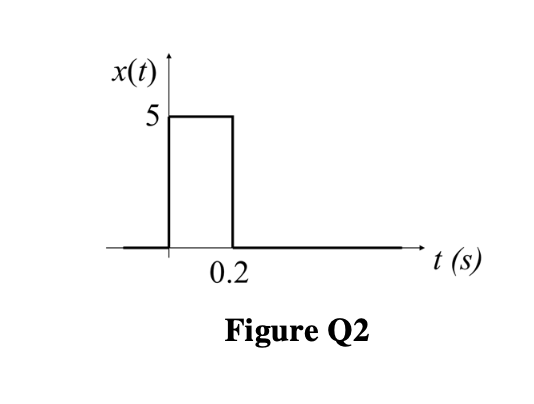
\includegraphics[width=0.3\textwidth]{images/Figure-Q2.png}

{[}6 marks{]}

    \begin{center}\rule{0.5\linewidth}{0.5pt}\end{center}

To develop the Fourier Transform \(X(f)\) of the signal \(x(t)\)
illustrated in the figure, we follow the same steps for a rectangular
pulse.

\paragraph{Step 1: Signal Description}\label{step-1-signal-description}

The signal \(x(t)\) is defined as: \[
x(t) =
\begin{cases} 
5, & 0 \leq t \leq 0.2, \\
0, & \text{otherwise}.
\end{cases}
\]

\paragraph{Step 2: Fourier Transform
Definition}\label{step-2-fourier-transform-definition}

The Fourier Transform is given by:
\(X(f) = \int_{-\infty}^\infty x(t) e^{-j 2 \pi f t} dt.\)

Since \(x(t)\) is nonzero only in the interval \([0, 0.2]\), the limits
of integration reduce to \([0, 0.2]\):
\(X(f) = \int_0^{0.2} 5 e^{-j 2 \pi f t} dt.\)

\paragraph{Step 3: Evaluate the
Integral}\label{step-3-evaluate-the-integral}

Factor out the constant \(5\):
\(X(f) = 5 \int_0^{0.2} e^{-j 2 \pi f t} dt.\)

The integral of \(e^{-j 2 \pi f t}\) is:
\(\int e^{-j 2 \pi f t} dt = \frac{e^{-j 2 \pi f t}}{-j 2 \pi f}.\)

Apply the limits of integration:
\(X(f) = 5 \left[ \frac{e^{-j 2 \pi f t}}{-j 2 \pi f} \right]_0^{0.2}.\)

Substitute the limits:
\(X(f) = 5 \cdot \frac{1}{-j 2 \pi f} \left( e^{-j 2 \pi f (0.2)} - e^{0} \right).\)

Simplify:
\(X(f) = \frac{5}{-j 2 \pi f} \left( e^{-j 0.4 \pi f} - 1 \right).\)

\paragraph{Step 4: Simplify Further}\label{step-4-simplify-further}

\paragraph{\texorpdfstring{\textbf{Using the property
\(e^{-j\theta} - 1 = -2j \sin\left(\frac{\theta}{2}\right) e^{-j\frac{\theta}{2}}\)}
which is derived as
follows:}{Using the property e\^{}\{-j\textbackslash theta\} - 1 = -2j \textbackslash sin\textbackslash left(\textbackslash frac\{\textbackslash theta\}\{2\}\textbackslash right) e\^{}\{-j\textbackslash frac\{\textbackslash theta\}\{2\}\} which is derived as follows:}}\label{using-the-property-e-jtheta---1--2j-sinleftfractheta2right-e-jfractheta2-which-is-derived-as-follows}

\begin{enumerate}
\def\labelenumi{\arabic{enumi}.}
\item
  \textbf{Rewrite \(e^{-j\theta} - 1\):} Expand using Euler's formula:
  \(e^{-j\theta} - 1 = \cos(\theta) - j\sin(\theta) - 1 =  (\cos(\theta) -1 ) - j\sin(\theta)\)
\item
  \textbf{Factorize Trigonometric Terms:} Use the half-angle identities:

  \begin{itemize}
  \tightlist
  \item
    \(\cos(\theta) = 1 -2\sin^2\left(\frac{\theta}{2}\right) \implies  \cos(\theta) - 1 = \color{orange}-2\sin^2\left(\frac{\theta}{2}\right)\)
  \item
    \(\sin(\theta) = \color{cyan}2\sin\left(\frac{\theta}{2}\right)\cos\left(\frac{\theta}{2}\right)\).
  \end{itemize}

  Substituting these:
  \(e^{-j\theta} - 1 = {\color{orange}-2\sin^2\left(\frac{\theta}{2}\right)} - j {\color{cyan}\cdot 2\sin\left(\frac{\theta}{2}\right)\cos\left(\frac{\theta}{2}\right)}.\)
\item
  \textbf{Factor Out Common Terms:}
\end{enumerate}

\begin{itemize}
\item
  \textbf{Identify Common Factor:}

  Both terms contain \(-2j\sin\left(\frac{\theta}{2}\right)\) as a
  common factor: 1. \(-2\sin^2\left(\frac{\theta}{2}\right)\): - This
  can be written as
  \(-2j\sin\left(\frac{\theta}{2}\right) \cdot \frac{\sin\left(\frac{\theta}{2}\right)}{j}\).
  2.
  \(-j \cdot 2\sin\left(\frac{\theta}{2}\right)\cos\left(\frac{\theta}{2}\right)\):
  - This is already proportional to
  \(-2j\sin\left(\frac{\theta}{2}\right)\).
\item
  \textbf{Factorization:}

  Factor \(-2j\sin\left(\frac{\theta}{2}\right)\) out of the entire
  expression:
  \(e^{-j\theta} - 1 = -2j\sin\left(\frac{\theta}{2}\right) \cdot \left(\frac{\sin\left(\frac{\theta}{2}\right)}{j} + \cos\left(\frac{\theta}{2}\right)\right).\)

  Simplify the term :
  \(\frac{\sin\left(\frac{\theta}{2}\right)}{j} = -j\sin\left(\frac{\theta}{2}\right).\)
  Thus:
  \(e^{-j\theta} - 1 = -2j\sin\left(\frac{\theta}{2}\right) \cdot \left(\cos\left(\frac{\theta}{2}\right) - j\sin\left(\frac{\theta}{2}\right)\right).\)
\item
  \textbf{Recognize the Exponential Form:} The term
  \(\cos\left(\frac{\theta}{2}\right) - j\sin\left(\frac{\theta}{2}\right)\)
  is equivalent to \(e^{-j\frac{\theta}{2}}\), using Euler's formula.
\end{itemize}

\begin{enumerate}
\def\labelenumi{\arabic{enumi}.}
\setcounter{enumi}{4}
\tightlist
\item
  \textbf{Simplify:} Recognize the term in parentheses as
  \(e^{-j\frac{\theta}{2}}\):
  \(e^{-j\theta} - 1 = -2j \sin\left(\frac{\theta}{2}\right) e^{-j\frac{\theta}{2}}.\)
\end{enumerate}

This compactly combines the amplitude term
\(-2j \sin\left(\frac{\theta}{2}\right)\) and the phase shift
\(e^{-j\frac{\theta}{2}}\).

\paragraph{\texorpdfstring{\textbf{rewrite \(X(f)\)}
:}{rewrite X(f) :}}\label{rewrite-xf}

\begin{itemize}
\tightlist
\item
  \(X(f) = \frac{5}{-j 2 \pi f} \cdot -2j \sin(0.2 \pi f) e^{-j 0.2 \pi f}.\)
\end{itemize}

Cancel \(-j\) and simplify:
\(X(f) = \frac{5 \cdot 2 \sin(0.2 \pi f)}{2 \pi f} e^{-j 0.2 \pi f}.\)

Finally: \(X(f) = \frac{5 \sin(0.2 \pi f)}{\pi f} e^{-j 0.2 \pi f}.\)

\paragraph{Final Expression}\label{final-expression}

\begin{align*}
X(f) &= \frac{5 \sin(0.2 \pi f)}{\pi f} \cdot e^{-j 0.2 \pi f} \\
&= 5 \cdot \text{sinc}(0.2 f) \cdot e^{-j 0.2 \pi f}
\end{align*}

where the \textbf{sinc function} is defined as:
\(\text{sinc}(x) = \frac{\sin(\pi x)}{\pi x}.\)

\subparagraph{Interpretation}\label{interpretation}

\begin{itemize}
\tightlist
\item
  \textbf{\(\frac{\sin(0.2 \pi f)}{\pi f}\):} This is the sinc function,
  representing the frequency-domain shape of the rectangular pulse.
\item
  \textbf{\(e^{-j 0.2 \pi f}\):} This is a phase shift due to the
  non-centered nature of the pulse (starting at \(t = 0\)).
\end{itemize}

    \begin{tcolorbox}[breakable, size=fbox, boxrule=1pt, pad at break*=1mm,colback=cellbackground, colframe=cellborder]
\prompt{In}{incolor}{1}{\boxspacing}
\begin{Verbatim}[commandchars=\\\{\}]
\PY{k}{using}\PY{+w}{ }\PY{n}{FFTW}\PY{p}{,}\PY{+w}{ }\PY{n}{LinearAlgebra}\PY{p}{,}\PY{+w}{ }\PY{n}{Plots}\PY{p}{,}\PY{+w}{ }\PY{n}{LaTeXStrings}
\end{Verbatim}
\end{tcolorbox}

    \begin{tcolorbox}[breakable, size=fbox, boxrule=1pt, pad at break*=1mm,colback=cellbackground, colframe=cellborder]
\prompt{In}{incolor}{2}{\boxspacing}
\begin{Verbatim}[commandchars=\\\{\}]
\PY{n}{include}\PY{p}{(}\PY{l+s}{\PYZdq{}}\PY{l+s}{../modules/operations.jl}\PY{l+s}{\PYZdq{}}\PY{p}{)}\PY{p}{;}
\end{Verbatim}
\end{tcolorbox}

    \begin{tcolorbox}[breakable, size=fbox, boxrule=1pt, pad at break*=1mm,colback=cellbackground, colframe=cellborder]
\prompt{In}{incolor}{3}{\boxspacing}
\begin{Verbatim}[commandchars=\\\{\}]
\PY{c}{\PYZsh{} Define the unscaled sinc function}
\PY{n}{sinc\PYZus{}unscaled}\PY{p}{(}\PY{n}{x}\PY{o}{::}\PY{k+kt}{Real}\PY{p}{)}\PY{+w}{ }\PY{o}{=}\PY{+w}{ }\PY{n}{x}\PY{+w}{ }\PY{o}{==}\PY{+w}{ }\PY{l+m+mi}{0}\PY{+w}{ }\PY{o}{?}\PY{+w}{ }\PY{l+m+mf}{1.0}\PY{+w}{ }\PY{o}{:}\PY{+w}{ }\PY{n}{sin}\PY{p}{(}\PY{n+nb}{pi}\PY{+w}{ }\PY{o}{*}\PY{+w}{ }\PY{n}{x}\PY{p}{)}\PY{+w}{ }\PY{o}{/}\PY{+w}{ }\PY{p}{(}\PY{n+nb}{pi}\PY{+w}{ }\PY{o}{*}\PY{+w}{ }\PY{n}{x}\PY{p}{)}

\PY{c}{\PYZsh{} Define the polymorphic sinc function with a normalization option}
\PY{n}{sinc}\PY{p}{(}\PY{n}{x}\PY{o}{::}\PY{k+kt}{Real}\PY{p}{;}\PY{+w}{ }\PY{n}{normalized}\PY{o}{::}\PY{k+kt}{Bool}\PY{+w}{ }\PY{o}{=}\PY{+w}{ }\PY{n+nb}{true}\PY{p}{)}\PY{+w}{ }\PY{o}{=}\PY{+w}{ }\PY{n}{normalized}\PY{+w}{ }\PY{o}{?}\PY{+w}{ }\PY{n}{sinc\PYZus{}unscaled}\PY{p}{(}\PY{n}{x}\PY{+w}{ }\PY{o}{/}\PY{+w}{ }\PY{n+nb}{π}\PY{p}{)}\PY{+w}{ }\PY{o}{:}\PY{+w}{ }\PY{n}{sinc\PYZus{}unscaled}\PY{p}{(}\PY{n}{x}\PY{p}{)}

\PY{c}{\PYZsh{} Frequency range}
\PY{n}{f}\PY{+w}{ }\PY{o}{=}\PY{+w}{ }\PY{n}{range}\PY{p}{(}\PY{o}{\PYZhy{}}\PY{l+m+mi}{40}\PY{p}{,}\PY{+w}{ }\PY{l+m+mi}{40}\PY{p}{,}\PY{+w}{ }\PY{n}{length}\PY{o}{=}\PY{l+m+mi}{1000}\PY{p}{)}

\PY{c}{\PYZsh{} Function components}
\PY{n}{𝒜}\PY{+w}{ }\PY{o}{=}\PY{+w}{ }\PY{l+m+mi}{5}\PY{+w}{ }\PY{o}{.*}\PY{+w}{ }\PY{n}{sinc}\PY{o}{.}\PY{p}{(}\PY{l+m+mf}{0.2}\PY{+w}{ }\PY{o}{.*}\PY{+w}{ }\PY{n}{f}\PY{p}{)}\PY{+w}{  }\PY{c}{\PYZsh{} Amplitude of the signal}
\PY{n}{ϕ}\PY{+w}{ }\PY{o}{=}\PY{+w}{ }\PY{n+nb}{ℯ}\PY{o}{.\PYZca{}}\PY{+w}{ }\PY{p}{(}\PY{o}{\PYZhy{}}\PY{n}{j}\PY{+w}{ }\PY{o}{.*}\PY{+w}{ }\PY{l+m+mf}{0.2}\PY{n+nb}{π}\PY{+w}{ }\PY{o}{.*}\PY{+w}{ }\PY{n}{f}\PY{p}{)}\PY{+w}{  }\PY{c}{\PYZsh{} Phase shift}
\PY{n}{𝐗}\PY{+w}{ }\PY{o}{=}\PY{+w}{ }\PY{n}{𝒜}\PY{+w}{ }\PY{o}{.*}\PY{+w}{ }\PY{n}{ϕ}\PY{+w}{  }\PY{c}{\PYZsh{} Combined function}

\PY{c}{\PYZsh{} Plot with title, labels, and semi\PYZhy{}transparent grid}
\PY{n}{plot}\PY{p}{(}\PY{n}{f}\PY{p}{,}\PY{+w}{ }\PY{n}{real}\PY{o}{.}\PY{p}{(}\PY{n}{𝐗}\PY{p}{)}
\PY{+w}{    }\PY{p}{,}\PY{+w}{ }\PY{n}{label}\PY{o}{=}\PY{l+s}{\PYZdq{}}\PY{l+s}{Real Part}\PY{l+s}{\PYZdq{}}\PY{p}{,}\PY{+w}{ }\PY{n}{linestyle}\PY{o}{=}\PY{l+s+ss}{:solid}\PY{p}{,}\PY{+w}{ }\PY{n}{linewidth}\PY{o}{=}\PY{l+m+mi}{2}\PY{p}{,}\PY{+w}{ }\PY{n}{alpha}\PY{o}{=}\PY{l+m+mf}{0.8}\PY{p}{,}\PY{+w}{ }\PY{n}{size}\PY{+w}{ }\PY{o}{=}\PY{+w}{ }\PY{p}{(}\PY{l+m+mi}{600}\PY{p}{,}\PY{l+m+mi}{400}\PY{p}{)}
\PY{+w}{    }\PY{p}{,}\PY{+w}{ }\PY{n}{xlabel}\PY{o}{=}\PY{l+s}{\PYZdq{}}\PY{l+s}{Frequency }\PY{l+s}{\PYZdq{}}\PY{+w}{ }\PY{o}{*}\PY{+w}{ }\PY{l+s+sa}{L}\PY{l+s}{\PYZdq{}}\PY{l+s}{f}\PY{l+s}{\PYZdq{}}\PY{p}{,}\PY{+w}{ }\PY{n}{ylabel}\PY{o}{=}\PY{l+s}{\PYZdq{}}\PY{l+s}{Amplitude}\PY{l+s}{\PYZdq{}}
\PY{+w}{    }\PY{p}{,}\PY{+w}{ }\PY{n}{title}\PY{o}{=}\PY{l+s}{\PYZdq{}}\PY{l+s}{Plot of }\PY{l+s}{\PYZdq{}}\PY{+w}{ }\PY{o}{*}\PY{+w}{ }\PY{l+s+sa}{L}\PY{l+s}{\PYZdq{}}\PY{l+s}{\PYZbs{}}\PY{l+s}{mathbf\PYZob{}X\PYZcb{}(f) = 5 sinc(0.2 f) e\PYZca{}\PYZob{}\PYZhy{}j 0.2 π f\PYZcb{}}\PY{l+s}{\PYZdq{}}
\PY{+w}{    }\PY{p}{,}\PY{+w}{ }\PY{n}{grid}\PY{o}{=}\PY{n+nb}{true}\PY{p}{,}\PY{+w}{ }\PY{n}{gridalpha}\PY{o}{=}\PY{l+m+mf}{0.2}\PY{+w}{  }\PY{c}{\PYZsh{} Enable grid and set transparency}
\PY{+w}{    }\PY{p}{,}\PY{+w}{ }\PY{n}{framestyle}\PY{o}{=}\PY{l+s+ss}{:box}
\PY{p}{)}

\PY{c}{\PYZsh{} Overlay additional lines}
\PY{n}{plot!}\PY{p}{(}\PY{n}{f}\PY{p}{,}\PY{+w}{ }\PY{n}{imag}\PY{o}{.}\PY{p}{(}\PY{n}{𝐗}\PY{p}{)}\PY{p}{,}\PY{+w}{ }\PY{n}{label}\PY{o}{=}\PY{l+s}{\PYZdq{}}\PY{l+s}{Imaginary Part}\PY{l+s}{\PYZdq{}}\PY{p}{,}\PY{+w}{ }\PY{n}{linestyle}\PY{o}{=}\PY{l+s+ss}{:dash}\PY{p}{,}\PY{+w}{ }\PY{n}{linewidth}\PY{o}{=}\PY{l+m+mi}{2}\PY{p}{,}\PY{+w}{ }\PY{n}{alpha}\PY{o}{=}\PY{l+m+mf}{0.8}\PY{p}{)}
\PY{n}{plot!}\PY{p}{(}\PY{n}{f}\PY{p}{,}\PY{+w}{ }\PY{n}{abs}\PY{o}{.}\PY{p}{(}\PY{n}{𝐗}\PY{p}{)}\PY{p}{,}\PY{+w}{ }\PY{n}{label}\PY{o}{=}\PY{l+s}{\PYZdq{}}\PY{l+s}{Magnitude}\PY{l+s}{\PYZdq{}}\PY{p}{,}\PY{+w}{ }\PY{n}{linestyle}\PY{o}{=}\PY{l+s+ss}{:dot}\PY{p}{,}\PY{+w}{ }\PY{n}{linewidth}\PY{o}{=}\PY{l+m+mi}{2}\PY{p}{,}\PY{+w}{ }\PY{n}{alpha}\PY{o}{=}\PY{l+m+mf}{0.8}\PY{p}{)}
\end{Verbatim}
\end{tcolorbox}
 
            
\prompt{Out}{outcolor}{3}{}
    
    \begin{center}
    \adjustimage{max size={0.9\linewidth}{0.9\paperheight}}{MathEng2223_files/MathEng2223_8_0.pdf}
    \end{center}
    { \hspace*{\fill} \\}
    

    

    \section{A linear, time-invariant system has the following transfer
function:}\label{a-linear-time-invariant-system-has-the-following-transfer-function}

\(H(s) = \frac{10(s + 100)}{s^2 + 2s + 100}\)

\begin{enumerate}
\def\labelenumi{(\alph{enumi})}
\item
  Derive an expression for \(H(s)\) in the usual, normal form.
\item
  Determine the frequency-invariant gain \(K\) and the position of any
  poles and zeros.
\item
  Sketch a Bode plot of the magnitude-frequency response.
\item
  Sketch a Bode plot of the phase-frequency response.
\end{enumerate}

{[}8 marks{]}

    \begin{center}\rule{0.5\linewidth}{0.5pt}\end{center}

\paragraph{\texorpdfstring{(a) Derive an expression for \(H(s)\) in the
usual, normal
form.}{(a) Derive an expression for H(s) in the usual, normal form.}}\label{a-derive-an-expression-for-hs-in-the-usual-normal-form.}

To derive the transfer function \(H(s)\) in the usual, \textbf{normal
form}, we factorize the numerator and denominator in terms of their
natural frequencies and damping ratios.

The given transfer function is:
\(H(s) = \frac{10(s + 100)}{s^2 + 2s + 100}.\)

\subparagraph{Step 1: Denominator Normal
Form}\label{step-1-denominator-normal-form}

The denominator is: \(s^2 + 2s + 100.\)

This matches the general form of a second-order system:
\(s^2 + 2\zeta\omega_n s + \omega_n^2,\) where \(\zeta\) is the damping
ratio and \(\omega_n\) is the natural frequency.

Here:
\(\omega_n^2 = 100 \quad \Rightarrow \quad \omega_n = \sqrt{100} = 10,\)
and:
\(2\zeta\omega_n = 2 \quad \Rightarrow \quad \zeta = \frac{2}{2\omega_n} = \frac{2}{20} = 0.1.\)

Thus, the denominator becomes:
\(s^2 + 2s + 100 = (s^2 + 2\zeta\omega_n s + \omega_n^2) = s^2 + 2(0.1)(10)s + 10^2.\)

\subparagraph{Step 2: Numerator Normal
Form}\label{step-2-numerator-normal-form}

The numerator is: \(10(s + 100).\)

Factor out \(100\) to normalize:
\(10(s + 100) = 10 \cdot 100 \left( \frac{s}{100} + 1 \right) = 1000 \left( \frac{s}{100} + 1 \right).\)

\subparagraph{Step 3: Rewrite in Normal
Form}\label{step-3-rewrite-in-normal-form}

Substitute the factored numerator and denominator into \(H(s)\):
\[H(s) = \frac{1000 \left( \frac{s}{100} + 1 \right)}{s^2 + 2(0.1)(10)s + 10^2}.\]

Simplify: \[
H(s) = \frac{1000}{100} \cdot \frac{\left( \frac{s}{100} + 1 \right)}{\frac{s^2}{100} + \frac{2(0.1)(10)s}{100} + \frac{10^2}{100}}.
\]

After normalization: \[
H(s) = \frac{10 \left( \frac{s}{100} + 1 \right)}{\frac{s^2}{100} + \frac{2s}{10} + 1}.
\]

Alternatively: \[
H(s) = \frac{10 \left( \frac{s}{100} + 1 \right)}{\frac{s^2}{100} + \frac{s}{5} + 1}.
\]

This is the normalized form of \(H(s)\).

    \paragraph{\texorpdfstring{(b): Determine the Frequency-Invariant Gain
\(K\) and the Positions of Poles and
Zeros}{(b): Determine the Frequency-Invariant Gain K and the Positions of Poles and Zeros}}\label{b-determine-the-frequency-invariant-gain-k-and-the-positions-of-poles-and-zeros}

\subparagraph{\texorpdfstring{1. \textbf{Transfer
Function}}{1. Transfer Function}}\label{transfer-function}

The given transfer function is:
\(H(s) = \frac{10(s + 100)}{s^2 + 2s + 100}.\)

\subparagraph{\texorpdfstring{2. \textbf{Frequency-Invariant Gain
\(K\)}}{2. Frequency-Invariant Gain K}}\label{frequency-invariant-gain-k}

The frequency-invariant gain is the gain of the system as \(s \to 0\).
This is determined by evaluating the transfer function at \(s = 0\): \[
K = H(0) = \frac{10(0 + 100)}{(0)^2 + 2(0) + 100}.
\]

Simplify: \(K = \frac{10 \cdot 100}{100} = 10.\)

Thus, the frequency-invariant gain is: \(K = 10.\)

\subparagraph{\texorpdfstring{3. \textbf{Poles}}{3. Poles}}\label{poles}

The poles are the roots of the denominator \(s^2 + 2s + 100 = 0\):
\(s^2 + 2s + 100 = 0.\)

Solve using the quadratic formula:
\(s = \frac{-b \pm \sqrt{b^2 - 4ac}}{2a},\) where \(a = 1\), \(b = 2\),
and \(c = 100\). Substituting:
\(s = \frac{-2 \pm \sqrt{2^2 - 4(1)(100)}}{2(1)} = \frac{-2 \pm \sqrt{4 - 400}}{2}.\)

Simplify: \(s = \frac{-2 \pm \sqrt{-396}}{2}.\)

The roots are: \(s = -1 \pm j\sqrt{99}.\)

Thus, the poles are: \(s = -1 + j\sqrt{99}, \quad s = -1 - j\sqrt{99}.\)

\subparagraph{\texorpdfstring{4. \textbf{Zeros}}{4. Zeros}}\label{zeros}

The zero is the root of the numerator \(10(s + 100) = 0\):
\(s + 100 = 0 \quad \Rightarrow \quad s = -100.\)

Thus, there is one zero at: \(s = -100.\)

\paragraph{Final Results:}\label{final-results}

\begin{itemize}
\item
  \textbf{Frequency-Invariant Gain \(K\):} \(K = 10.\)
\item
  \textbf{Poles:} \(s = -1 + j\sqrt{99}, \quad s = -1 - j\sqrt{99}.\)
\item
  \textbf{Zero:} \(s = -100.\)
\end{itemize}

    \begin{tcolorbox}[breakable, size=fbox, boxrule=1pt, pad at break*=1mm,colback=cellbackground, colframe=cellborder]
\prompt{In}{incolor}{4}{\boxspacing}
\begin{Verbatim}[commandchars=\\\{\}]
\PY{c}{\PYZsh{} Frequency range (logarithmic scale)}
\PY{n}{ω}\PY{+w}{ }\PY{o}{=}\PY{+w}{ }\PY{l+m+mi}{10}\PY{+w}{ }\PY{o}{.\PYZca{}}\PY{+w}{ }\PY{n}{range}\PY{p}{(}\PY{o}{\PYZhy{}}\PY{l+m+mi}{1}\PY{p}{,}\PY{+w}{ }\PY{l+m+mi}{3}\PY{p}{,}\PY{+w}{ }\PY{n}{length}\PY{o}{=}\PY{l+m+mi}{500}\PY{p}{)}\PY{+w}{  }\PY{c}{\PYZsh{} Frequencies from 0.1 to 1000 (log scale)}

\PY{c}{\PYZsh{} Define the transfer function H(s)}
\PY{k}{function}\PY{+w}{ }\PY{n}{H}\PY{p}{(}\PY{n}{ω}\PY{p}{)}
\PY{+w}{    }\PY{n}{numerator}\PY{+w}{ }\PY{o}{=}\PY{+w}{ }\PY{l+m+mi}{10}\PY{+w}{ }\PY{o}{.*}\PY{+w}{ }\PY{p}{(}\PY{n}{j}\PY{+w}{ }\PY{o}{.*}\PY{+w}{ }\PY{n}{ω}\PY{+w}{ }\PY{o}{.+}\PY{+w}{ }\PY{l+m+mi}{100}\PY{p}{)}\PY{+w}{  }\PY{c}{\PYZsh{} Element\PYZhy{}wise addition}
\PY{+w}{    }\PY{n}{denominator}\PY{+w}{ }\PY{o}{=}\PY{+w}{ }\PY{p}{(}\PY{n}{j}\PY{+w}{ }\PY{o}{.*}\PY{+w}{ }\PY{n}{ω}\PY{p}{)}\PY{o}{.\PYZca{}}\PY{l+m+mi}{2}\PY{+w}{ }\PY{o}{.+}\PY{+w}{ }\PY{l+m+mi}{2}\PY{+w}{ }\PY{o}{.*}\PY{+w}{ }\PY{p}{(}\PY{n}{j}\PY{+w}{ }\PY{o}{.*}\PY{+w}{ }\PY{n}{ω}\PY{p}{)}\PY{+w}{ }\PY{o}{.+}\PY{+w}{ }\PY{l+m+mi}{100}\PY{+w}{  }\PY{c}{\PYZsh{} Element\PYZhy{}wise operations}
\PY{+w}{    }\PY{k}{return}\PY{+w}{ }\PY{n}{numerator}\PY{+w}{ }\PY{o}{./}\PY{+w}{ }\PY{n}{denominator}\PY{+w}{  }\PY{c}{\PYZsh{} Element\PYZhy{}wise division}
\PY{k}{end}
\end{Verbatim}
\end{tcolorbox}

            \begin{tcolorbox}[breakable, size=fbox, boxrule=.5pt, pad at break*=1mm, opacityfill=0]
\prompt{Out}{outcolor}{4}{\boxspacing}
\begin{Verbatim}[commandchars=\\\{\}]
H (generic function with 1 method)
\end{Verbatim}
\end{tcolorbox}
        
    \begin{tcolorbox}[breakable, size=fbox, boxrule=1pt, pad at break*=1mm,colback=cellbackground, colframe=cellborder]
\prompt{In}{incolor}{5}{\boxspacing}
\begin{Verbatim}[commandchars=\\\{\}]
\PY{k}{using}\PY{+w}{ }\PY{n}{Plots}
\PY{k}{using}\PY{+w}{ }\PY{n}{Printf}
\PY{k}{using}\PY{+w}{ }\PY{n}{Measures}

\PY{c}{\PYZsh{} Magnitude response in dB}
\PY{n}{magnitude\PYZus{}dB}\PY{+w}{ }\PY{o}{=}\PY{+w}{ }\PY{l+m+mi}{20}\PY{+w}{ }\PY{o}{.*}\PY{+w}{ }\PY{n}{log10}\PY{o}{.}\PY{p}{(}\PY{n}{abs}\PY{o}{.}\PY{p}{(}\PY{n}{H}\PY{o}{.}\PY{p}{(}\PY{n}{ω}\PY{p}{)}\PY{p}{)}\PY{p}{)}\PY{+w}{  }\PY{c}{\PYZsh{} Broadcasting applied to H, abs, and log10}

\PY{c}{\PYZsh{} Plot the Bode magnitude plot}
\PY{n}{p1}\PY{+w}{ }\PY{o}{=}\PY{+w}{ }\PY{n}{plot}\PY{p}{(}\PY{n}{ω}\PY{p}{,}\PY{+w}{ }\PY{n}{magnitude\PYZus{}dB}
\PY{+w}{    }\PY{p}{,}\PY{+w}{ }\PY{n}{xscale}\PY{o}{=}\PY{l+s+ss}{:log10}
\PY{+w}{    }\PY{p}{,}\PY{+w}{ }\PY{n}{xlabel}\PY{o}{=}\PY{l+s}{\PYZdq{}}\PY{l+s}{Frequency (rad/s)}\PY{l+s}{\PYZdq{}}\PY{p}{,}\PY{+w}{ }\PY{n}{ylabel}\PY{o}{=}\PY{l+s}{\PYZdq{}}\PY{l+s}{Magnitude (dB)}\PY{l+s}{\PYZdq{}}
\PY{+w}{    }\PY{p}{,}\PY{+w}{ }\PY{n}{title}\PY{o}{=}\PY{l+s}{\PYZdq{}}\PY{l+s}{Bode Magnitude Plot}\PY{l+s}{\PYZdq{}}\PY{p}{,}\PY{+w}{ }\PY{n}{legend}\PY{o}{=}\PY{n+nb}{false}\PY{p}{,}\PY{+w}{ }\PY{n}{grid}\PY{o}{=}\PY{n+nb}{true}
\PY{+w}{    }\PY{p}{,}\PY{+w}{ }\PY{n}{margin}\PY{+w}{ }\PY{o}{=}\PY{+w}{ }\PY{l+m+mi}{5}\PY{n}{mm}
\PY{p}{)}

\PY{c}{\PYZsh{} Phase response in degrees}
\PY{n}{phase\PYZus{}deg}\PY{+w}{ }\PY{o}{=}\PY{+w}{ }\PY{n}{angle}\PY{o}{.}\PY{p}{(}\PY{n}{H}\PY{o}{.}\PY{p}{(}\PY{n}{ω}\PY{p}{)}\PY{p}{)}\PY{+w}{ }\PY{o}{.*}\PY{+w}{ }\PY{p}{(}\PY{l+m+mi}{180}\PY{+w}{ }\PY{o}{/}\PY{+w}{ }\PY{n+nb}{π}\PY{p}{)}\PY{+w}{  }\PY{c}{\PYZsh{} Convert phase from radians to degrees}

\PY{c}{\PYZsh{} Plot the Bode phase plot}
\PY{n}{p2}\PY{+w}{ }\PY{o}{=}\PY{+w}{ }\PY{n}{plot}\PY{p}{(}\PY{n}{ω}\PY{p}{,}\PY{+w}{ }\PY{n}{phase\PYZus{}deg}
\PY{+w}{    }\PY{p}{,}\PY{n}{xscale}\PY{o}{=}\PY{l+s+ss}{:log10}
\PY{+w}{    }\PY{p}{,}\PY{n}{xlabel}\PY{o}{=}\PY{l+s}{\PYZdq{}}\PY{l+s}{Frequency (rad/s)}\PY{l+s}{\PYZdq{}}\PY{p}{,}\PY{+w}{ }\PY{n}{ylabel}\PY{o}{=}\PY{l+s}{\PYZdq{}}\PY{l+s}{Phase (degrees)}\PY{l+s}{\PYZdq{}}
\PY{+w}{    }\PY{p}{,}\PY{n}{title}\PY{o}{=}\PY{l+s}{\PYZdq{}}\PY{l+s}{Bode Phase Plot}\PY{l+s}{\PYZdq{}}
\PY{+w}{    }\PY{p}{,}\PY{n}{legend}\PY{o}{=}\PY{n+nb}{false}\PY{p}{,}\PY{n}{grid}\PY{o}{=}\PY{n+nb}{true}
\PY{+w}{    }\PY{p}{,}\PY{n}{left\PYZus{}margin}\PY{o}{=}\PY{l+m+mi}{10}\PY{n}{mm}\PY{p}{,}\PY{+w}{ }\PY{n}{right\PYZus{}margin}\PY{o}{=}\PY{l+m+mi}{10}\PY{n}{mm}\PY{p}{,}\PY{+w}{ }\PY{n}{top\PYZus{}margin}\PY{o}{=}\PY{l+m+mi}{15}\PY{n}{mm}\PY{p}{,}\PY{+w}{ }\PY{n}{bottom\PYZus{}margin}\PY{o}{=}\PY{l+m+mi}{15}\PY{n}{mm}
\PY{p}{)}

\PY{n}{plot}\PY{p}{(}\PY{n}{p1}\PY{p}{,}\PY{+w}{ }\PY{n}{p2}\PY{p}{,}\PY{+w}{ }\PY{n}{layout}\PY{+w}{ }\PY{o}{=}\PY{+w}{ }\PY{p}{(}\PY{l+m+mi}{1}\PY{p}{,}\PY{+w}{ }\PY{l+m+mi}{2}\PY{p}{)}\PY{p}{,}\PY{+w}{ }\PY{n}{size}\PY{+w}{ }\PY{o}{=}\PY{+w}{ }\PY{p}{(}\PY{l+m+mi}{1000}\PY{p}{,}\PY{+w}{ }\PY{l+m+mi}{400}\PY{p}{)}\PY{p}{)}
\end{Verbatim}
\end{tcolorbox}
 
            
\prompt{Out}{outcolor}{5}{}
    
    \begin{center}
    \adjustimage{max size={0.9\linewidth}{0.9\paperheight}}{MathEng2223_files/MathEng2223_14_0.pdf}
    \end{center}
    { \hspace*{\fill} \\}
    

    \section{Sketch magnitude and phase responses for a sampled data system
with a pair of complex conjugate zeros and two poles at the
origin.}\label{sketch-magnitude-and-phase-responses-for-a-sampled-data-system-with-a-pair-of-complex-conjugate-zeros-and-two-poles-at-the-origin.}

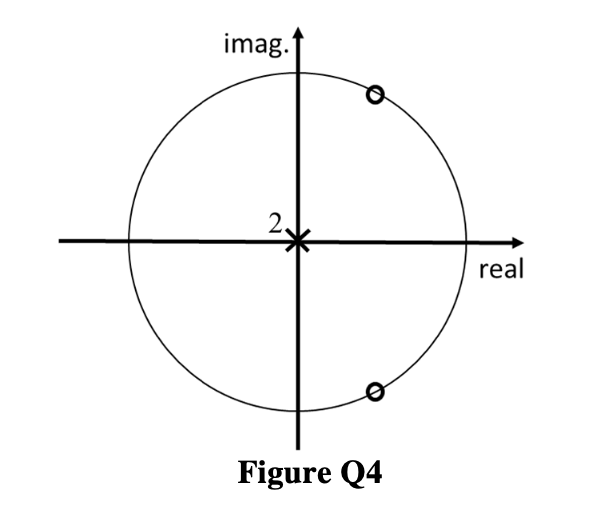
\includegraphics[width=0.3\textwidth]{images/Figure-Q4.png}

{[}4 marks{]}

    The question asks for magnitude and phase response plots for a sampled
data system with:

\begin{enumerate}
\def\labelenumi{\arabic{enumi}.}
\tightlist
\item
  \textbf{Two complex conjugate zeros} located on the unit circle.
\item
  \textbf{Two poles at the origin}.
\end{enumerate}

This indicates a discrete-time system, and we can describe the transfer
function in the z-domain.

\paragraph{Step 1: Transfer Function
Representation}\label{step-1-transfer-function-representation}

From the given information:

\begin{itemize}
\item
  \textbf{Zeros:} The system has complex conjugate zeros located on the
  unit circle at \(z = e^{j\theta}\) and \(z = e^{-j\theta}\). For
  simplicity, let the zeros be at \(z = e^{j\pi/4}\) and
  \(z = e^{-j\pi/4}\).
\item
  \textbf{Poles:} Two poles are at the origin (\(z = 0\)).
\end{itemize}

The transfer function is: \[
H(z) = K \frac{(z - e^{j\pi/4})(z - e^{-j\pi/4})}{z^2},
\] where \(K\) is the gain.

Simplify the numerator using the property of complex conjugates:
\((z - e^{j\pi/4})(z - e^{-j\pi/4}) = z^2 - 2z\cos(\pi/4) + 1 = z^2 - \sqrt{2}z + 1.\)

Thus, the transfer function becomes:
\(H(z) = K \frac{z^2 - \sqrt{2}z + 1}{z^2}.\)

\paragraph{Step 2: Frequency Response}\label{step-2-frequency-response}

Substitute \(z = e^{j\omega}\) (discrete-time frequency variable):

\(H(e^{j\omega}) = K \frac{e^{2j\omega} - \sqrt{2}e^{j\omega} + 1}{e^{2j\omega}}.\)

Simplify:
\(H(e^{j\omega}) = K \left( 1 - \sqrt{2}e^{-j\omega} + e^{-2j\omega} \right).\)

The magnitude response is:
\(|H(e^{j\omega})| = |K| \cdot \left| 1 - \sqrt{2}e^{-j\omega} + e^{-2j\omega} \right|.\)

The phase response is:
\(\text{Phase}(H(e^{j\omega})) = \arg\left( 1 - \sqrt{2}e^{-j\omega} + e^{-2j\omega} \right).\)

\paragraph{Step 3: Magnitude and Phase Plot
Characteristics}\label{step-3-magnitude-and-phase-plot-characteristics}

\begin{enumerate}
\def\labelenumi{\arabic{enumi}.}
\tightlist
\item
  \textbf{Magnitude Response:}

  \begin{itemize}
  \tightlist
  \item
    Peaks occur near the frequencies corresponding to the zeros (here,
    \(\pi/4\) and \(-\pi/4\)).
  \item
    High attenuation occurs near the poles (low frequencies), since the
    poles are at the origin.
  \end{itemize}
\item
  \textbf{Phase Response:}

  \begin{itemize}
  \tightlist
  \item
    The phase changes rapidly near the frequencies of the zeros.
  \item
    At low frequencies, the phase starts at \(0^\circ\) due to the
    dominance of the poles.
  \end{itemize}
\end{enumerate}

\paragraph{Step 4: Sketch the Plots}\label{step-4-sketch-the-plots}

Here's how the plots would look:

\begin{enumerate}
\def\labelenumi{\arabic{enumi}.}
\tightlist
\item
  \textbf{Magnitude Plot:}

  \begin{itemize}
  \tightlist
  \item
    Start at low values near \(\omega = 0\) (due to the poles).
  \item
    Peaks occur near \(\omega = \pi/4\) and \(\omega = -\pi/4\)
    (locations of the zeros).
  \item
    Symmetrical around \(\omega = 0\).
  \end{itemize}
\item
  \textbf{Phase Plot:}

  \begin{itemize}
  \tightlist
  \item
    At \(\omega = 0\), the phase is \(0^\circ\).
  \item
    The phase decreases sharply near \(\omega = \pi/4\) and
    \(\omega = -\pi/4\).
  \end{itemize}
\end{enumerate}

    \begin{tcolorbox}[breakable, size=fbox, boxrule=1pt, pad at break*=1mm,colback=cellbackground, colframe=cellborder]
\prompt{In}{incolor}{6}{\boxspacing}
\begin{Verbatim}[commandchars=\\\{\}]
\PY{k}{using}\PY{+w}{ }\PY{n}{Plots}
\PY{k}{using}\PY{+w}{ }\PY{n}{Printf}

\PY{c}{\PYZsh{} Define the transfer function H(e\PYZca{}jw) for the discrete\PYZhy{}time system}
\PY{k}{function}\PY{+w}{ }\PY{n}{H}\PY{p}{(}\PY{n}{ω}\PY{p}{)}
\PY{+w}{    }\PY{c}{\PYZsh{} Complex exponential terms}
\PY{+w}{    }\PY{n}{z₁}\PY{+w}{ }\PY{o}{=}\PY{+w}{ }\PY{n+nb}{ℯ}\PY{o}{\PYZca{}}\PY{p}{(}\PY{o}{\PYZhy{}}\PY{n}{j}\PY{+w}{ }\PY{o}{*}\PY{+w}{ }\PY{n}{ω}\PY{p}{)}\PY{+w}{  }\PY{c}{\PYZsh{} e\PYZca{}(jω)}
\PY{+w}{    }\PY{n}{z₂}\PY{+w}{ }\PY{o}{=}\PY{+w}{ }\PY{n+nb}{ℯ}\PY{o}{\PYZca{}}\PY{p}{(}\PY{o}{\PYZhy{}}\PY{l+m+mi}{2}\PY{n}{j}\PY{+w}{ }\PY{o}{*}\PY{+w}{ }\PY{n}{ω}\PY{p}{)}\PY{+w}{  }\PY{c}{\PYZsh{} e\PYZca{}(j2ω)}

\PY{+w}{    }\PY{c}{\PYZsh{} Transfer function}
\PY{+w}{    }\PY{n}{numerator}\PY{+w}{ }\PY{o}{=}\PY{+w}{ }\PY{n}{z₂}\PY{o}{\PYZca{}}\PY{l+m+mi}{2}\PY{+w}{ }\PY{o}{\PYZhy{}}\PY{+w}{ }\PY{o}{√}\PY{p}{(}\PY{l+m+mi}{2}\PY{p}{)}\PY{+w}{ }\PY{o}{*}\PY{+w}{ }\PY{n}{z₁}\PY{+w}{ }\PY{o}{+}\PY{+w}{ }\PY{l+m+mi}{1}\PY{+w}{  }\PY{c}{\PYZsh{} (z\PYZca{}2 \PYZhy{} sqrt(2)z + 1)}
\PY{+w}{    }\PY{n}{denominator}\PY{+w}{ }\PY{o}{=}\PY{+w}{ }\PY{n}{z₂}\PY{o}{\PYZca{}}\PY{l+m+mi}{2}\PY{+w}{  }\PY{c}{\PYZsh{} (z\PYZca{}2)}
\PY{+w}{    }\PY{k}{return}\PY{+w}{ }\PY{n}{numerator}\PY{+w}{ }\PY{o}{/}\PY{+w}{ }\PY{n}{denominator}
\PY{k}{end}

\PY{c}{\PYZsh{} Frequency range (from \PYZhy{}π to π for discrete systems)}
\PY{n}{ω}\PY{+w}{ }\PY{o}{=}\PY{+w}{ }\PY{n}{range}\PY{p}{(}\PY{o}{\PYZhy{}}\PY{n+nb}{π}\PY{p}{,}\PY{+w}{ }\PY{n+nb}{π}\PY{p}{,}\PY{+w}{ }\PY{n}{length}\PY{o}{=}\PY{l+m+mi}{500}\PY{p}{)}

\PY{c}{\PYZsh{} Magnitude response}
\PY{n}{magnitude}\PY{+w}{ }\PY{o}{=}\PY{+w}{ }\PY{n}{abs}\PY{o}{.}\PY{p}{(}\PY{n}{H}\PY{o}{.}\PY{p}{(}\PY{n}{ω}\PY{p}{)}\PY{p}{)}
\PY{n}{magnitude\PYZus{}dB}\PY{+w}{ }\PY{o}{=}\PY{+w}{ }\PY{l+m+mi}{20}\PY{+w}{ }\PY{o}{.*}\PY{+w}{ }\PY{n}{log10}\PY{o}{.}\PY{p}{(}\PY{n}{magnitude}\PY{p}{)}\PY{+w}{  }\PY{c}{\PYZsh{} Convert to dB}

\PY{c}{\PYZsh{} Phase response}
\PY{n}{phase}\PY{+w}{ }\PY{o}{=}\PY{+w}{ }\PY{n}{angle}\PY{o}{.}\PY{p}{(}\PY{n}{H}\PY{o}{.}\PY{p}{(}\PY{n}{ω}\PY{p}{)}\PY{p}{)}\PY{+w}{ }\PY{o}{.*}\PY{+w}{ }\PY{p}{(}\PY{l+m+mi}{180}\PY{+w}{ }\PY{o}{/}\PY{+w}{ }\PY{n+nb}{π}\PY{p}{)}\PY{+w}{  }\PY{c}{\PYZsh{} Convert radians to degrees}

\PY{c}{\PYZsh{} Plot the magnitude response}
\PY{n}{p1}\PY{+w}{ }\PY{o}{=}\PY{+w}{ }\PY{n}{plot}\PY{p}{(}
\PY{+w}{    }\PY{n}{ω}\PY{p}{,}\PY{+w}{ }\PY{n}{magnitude\PYZus{}dB}\PY{p}{,}
\PY{+w}{    }\PY{n}{xlabel}\PY{o}{=}\PY{l+s}{\PYZdq{}}\PY{l+s}{Frequency (rad/sample)}\PY{l+s}{\PYZdq{}}\PY{p}{,}
\PY{+w}{    }\PY{n}{ylabel}\PY{o}{=}\PY{l+s}{\PYZdq{}}\PY{l+s}{Magnitude (dB)}\PY{l+s}{\PYZdq{}}\PY{p}{,}
\PY{+w}{    }\PY{n}{title}\PY{o}{=}\PY{l+s}{\PYZdq{}}\PY{l+s}{Bode Magnitude Plot}\PY{l+s}{\PYZdq{}}\PY{p}{,}
\PY{+w}{    }\PY{n}{legend}\PY{o}{=}\PY{n+nb}{false}\PY{p}{,}
\PY{+w}{    }\PY{n}{grid}\PY{o}{=}\PY{n+nb}{true}
\PY{p}{)}

\PY{c}{\PYZsh{} Plot the phase response}
\PY{n}{p2}\PY{+w}{ }\PY{o}{=}\PY{+w}{ }\PY{n}{plot}\PY{p}{(}
\PY{+w}{    }\PY{n}{ω}\PY{p}{,}\PY{+w}{ }\PY{n}{phase}\PY{p}{,}
\PY{+w}{    }\PY{n}{xlabel}\PY{o}{=}\PY{l+s}{\PYZdq{}}\PY{l+s}{Frequency (rad/sample)}\PY{l+s}{\PYZdq{}}\PY{p}{,}
\PY{+w}{    }\PY{n}{ylabel}\PY{o}{=}\PY{l+s}{\PYZdq{}}\PY{l+s}{Phase (degrees)}\PY{l+s}{\PYZdq{}}\PY{p}{,}
\PY{+w}{    }\PY{n}{title}\PY{o}{=}\PY{l+s}{\PYZdq{}}\PY{l+s}{Bode Phase Plot}\PY{l+s}{\PYZdq{}}\PY{p}{,}
\PY{+w}{    }\PY{n}{legend}\PY{o}{=}\PY{n+nb}{false}\PY{p}{,}
\PY{+w}{    }\PY{n}{grid}\PY{o}{=}\PY{n+nb}{true}
\PY{p}{)}

\PY{n}{plot}\PY{p}{(}\PY{n}{p1}\PY{p}{,}\PY{n}{p2}\PY{p}{,}\PY{n}{layout}\PY{+w}{ }\PY{o}{=}\PY{+w}{ }\PY{p}{(}\PY{l+m+mi}{2}\PY{p}{,}\PY{l+m+mi}{1}\PY{p}{)}\PY{p}{)}
\end{Verbatim}
\end{tcolorbox}
 
            
\prompt{Out}{outcolor}{6}{}
    
    \begin{center}
    \adjustimage{max size={0.9\linewidth}{0.9\paperheight}}{MathEng2223_files/MathEng2223_17_0.pdf}
    \end{center}
    { \hspace*{\fill} \\}
    

    \section{\texorpdfstring{A random variable \(X\) is uniformly
distributed between \(x = 0\) and \(x = 1\). Via any appropriate method,
determine the expected value \(E[Y]\) of
\(Y = exp(X)\).}{A random variable X is uniformly distributed between x = 0 and x = 1. Via any appropriate method, determine the expected value E{[}Y{]} of Y = exp(X).}}\label{a-random-variable-x-is-uniformly-distributed-between-x-0-and-x-1.-via-any-appropriate-method-determine-the-expected-value-ey-of-y-expx.}

{[}4 marks{]}

    \begin{center}\rule{0.5\linewidth}{0.5pt}\end{center}

Given \(Y = \exp(X)\) and \(X \sim U(0, 1)\),

\paragraph{\texorpdfstring{\textbf{1. Expected Value
Formula}}{1. Expected Value Formula}}\label{expected-value-formula}

The expected value of a random variable \(Y\) is given by:

\[E[Y] = \int_{-\infty}^\infty y f_Y(y) \, dy.\]

Since \(X\) is uniformly distributed, its probability density function
(PDF) is:

\[
f_X(x) = 
\begin{cases} 
1, & 0 \leq x \leq 1, \\
0, & \text{otherwise}.
\end{cases}
\]

For \(Y = \exp(X)\), the expected value becomes:
\(E[Y] = \int_0^1 \exp(x) f_X(x) \, dx.\)

Because \(f_X(x) = 1\)for\(0 \leq x \leq 1\), this simplifies to:
\(E[Y] = \int_0^1 \exp(x) \, dx.\)

\paragraph{\texorpdfstring{\textbf{2. Solve the
Integral}}{2. Solve the Integral}}\label{solve-the-integral}

The integral of \(\exp(x)\) is: \(\int \exp(x) \, dx = \exp(x) + C.\)

Now, evaluate the definite integral:
\(\int_0^1 \exp(x) \, dx = \left[ \exp(x) \right]_0^1 = \exp(1) - \exp(0).\)

Simplify: \(\int_0^1 \exp(x) \, dx = e - 1.\)

\paragraph{\texorpdfstring{\textbf{3. Final
Answer}}{3. Final Answer}}\label{final-answer}

The expected value is: \(\boxed{E[Y] = e - 1}\)

    \section{\texorpdfstring{Identify the pivots and free variables of the
following two matrices \(A\) and \(B\). Following the method which we
studied in class, find the special solution corresponding to each free
variable and, by combining the special solutions, describe every
solution to \(Ax=0\) and
\(Bx=0\).}{Identify the pivots and free variables of the following two matrices A and B. Following the method which we studied in class, find the special solution corresponding to each free variable and, by combining the special solutions, describe every solution to Ax=0 and Bx=0.}}\label{identify-the-pivots-and-free-variables-of-the-following-two-matrices-a-and-b.-following-the-method-which-we-studied-in-class-find-the-special-solution-corresponding-to-each-free-variable-and-by-combining-the-special-solutions-describe-every-solution-to-ax0-and-bx0.}

\[
A = 
\begin{bmatrix}
1 & 2 & 2 & 4 & 6 \\
1 & 2 & 3 & 6 & 9 \\
0 & 0 & 1 & 2 & 3
\end{bmatrix} \qquad \text{and} \quad
B = 
\begin{bmatrix}
2 & 4 & 2 \\
0 & 4 & 4 \\
0 & 8 & 8
\end{bmatrix}.
\]

{[}7 marks{]}

    \begin{center}\rule{0.5\linewidth}{0.5pt}\end{center}

To find the pivots, free variables, and solutions to \(Ax = 0\) and
\(Bx = 0\), we follow these steps:

\paragraph{\texorpdfstring{Step 1: Row Reduction of Matrix
\(A\)}{Step 1: Row Reduction of Matrix A}}\label{step-1-row-reduction-of-matrix-a}

Matrix \(A\) is: \[
A = 
\begin{bmatrix}
1 & 2 & 2 & 4 & 6 \\
1 & 2 & 3 & 6 & 9 \\
0 & 0 & 1 & 2 & 3
\end{bmatrix}.
\]

\subparagraph{\texorpdfstring{Row Reduce \(A\) to Row Echelon
Form}{Row Reduce A to Row Echelon Form}}\label{row-reduce-a-to-row-echelon-form}

\begin{enumerate}
\def\labelenumi{\arabic{enumi}.}
\item
  Subtract the first row from the second: \[
  \begin{bmatrix}
  1 & 2 & 2 & 4 & 6 \\
  0 & 0 & 1 & 2 & 3 \\
  0 & 0 & 1 & 2 & 3
  \end{bmatrix}.
  \]
\item
  Subtract the third row from the second: \[
  \begin{bmatrix}
  1 & 2 & 2 & 4 & 6 \\
  0 & 0 & 1 & 2 & 3 \\
  0 & 0 & 0 & 0 & 0
  \end{bmatrix}.
  \]
\end{enumerate}

\subparagraph{Identify Pivots and Free
Variables}\label{identify-pivots-and-free-variables}

\begin{itemize}
\tightlist
\item
  \textbf{Pivot columns}: The first column (\(x_1\)) and third column
  (\(x_3\)).
\item
  \textbf{Free variables}: The second column (\(x_2\)), fourth column
  (\(x_4\)), and fifth column (\(x_5\)).
\end{itemize}

\begin{center}\rule{0.5\linewidth}{0.5pt}\end{center}

\paragraph{\texorpdfstring{Step 2: Solve \(Ax = 0\) (Homogeneous
System)}{Step 2: Solve Ax = 0 (Homogeneous System)}}\label{step-2-solve-ax-0-homogeneous-system}

The system is represented as:

\[
\begin{aligned}
x_1 + 2x_2 + 2x_3 + 4x_4 + 6x_5 &= 0, \\
x_3 + 2x_4 + 3x_5 &= 0.
\end{aligned}
\]

\subparagraph{Back-Substitute:}\label{back-substitute}

\begin{enumerate}
\def\labelenumi{\arabic{enumi}.}
\item
  From the second equation: \(x_3 = -2x_4 - 3x_5.\)
\item
  Substitute \(x_3\) into the first equation:
  \(x_1 + 2x_2 + 2(-2x_4 - 3x_5) + 4x_4 + 6x_5 = 0,\)
  \(x_1 + 2x_2 - 4x_4 - 6x_5 + 4x_4 + 6x_5 = 0,\)
  \(x_1 + 2x_2 = 0 \implies x_1 = -2x_2.\)
\end{enumerate}

\subparagraph{\texorpdfstring{Write the General Solution for
\(Ax = 0\):}{Write the General Solution for Ax = 0:}}\label{write-the-general-solution-for-ax-0}

\[
x =
\begin{bmatrix}
x_1 \\ x_2 \\ x_3 \\ x_4 \\ x_5
\end{bmatrix} =
x_2
\begin{bmatrix}
-2 \\ 1 \\ 0 \\ 0 \\ 0
\end{bmatrix} +
x_4
\begin{bmatrix}
0 \\ 0 \\ -2 \\ 1 \\ 0
\end{bmatrix} +
x_5
\begin{bmatrix}
0 \\ 0 \\ -3 \\ 0 \\ 1
\end{bmatrix}.
\]

The \textbf{special solutions} correspond to the free variables \(x_2\),
\(x_4\), and \(x_5\).

\begin{center}\rule{0.5\linewidth}{0.5pt}\end{center}

\paragraph{\texorpdfstring{Step 3: Row Reduction of Matrix
\(B\)}{Step 3: Row Reduction of Matrix B}}\label{step-3-row-reduction-of-matrix-b}

Matrix \(B\) is: \[
B = 
\begin{bmatrix}
2 & 4 & 2 \\
0 & 4 & 4 \\
0 & 8 & 8
\end{bmatrix}.
\]

\subparagraph{\texorpdfstring{Row Reduce \(B\) to Row Echelon
Form}{Row Reduce B to Row Echelon Form}}\label{row-reduce-b-to-row-echelon-form}

\begin{enumerate}
\def\labelenumi{\arabic{enumi}.}
\item
  Divide the first row by 2: \[
  \begin{bmatrix}
  1 & 2 & 1 \\
  0 & 4 & 4 \\
  0 & 8 & 8
  \end{bmatrix}.
  \]
\item
  Divide the second row by 4: \[
  \begin{bmatrix}
  1 & 2 & 1 \\
  0 & 1 & 1 \\
  0 & 8 & 8
  \end{bmatrix}.
  \]
\item
  Subtract 8 times the second row from the third: \[
  \begin{bmatrix}
  1 & 2 & 1 \\
  0 & 1 & 1 \\
  0 & 0 & 0
  \end{bmatrix}.
  \]
\end{enumerate}

\subparagraph{Identify Pivots and Free
Variables}\label{identify-pivots-and-free-variables-1}

\begin{itemize}
\tightlist
\item
  \textbf{Pivot columns}: The first column (\(x_1\)) and the second
  column (\(x_2\)).
\item
  \textbf{Free variable}: The third column (\(x_3\)).
\end{itemize}

\paragraph{\texorpdfstring{Step 4: Solve \(Bx = 0\) (Homogeneous
System)}{Step 4: Solve Bx = 0 (Homogeneous System)}}\label{step-4-solve-bx-0-homogeneous-system}

The system is represented as: \[
\begin{aligned}
x_1 + 2x_2 + x_3 &= 0, \\
x_2 + x_3 &= 0.
\end{aligned}
\]

\subparagraph{Back-Substitute:}\label{back-substitute-1}

\begin{enumerate}
\def\labelenumi{\arabic{enumi}.}
\item
  From the second equation: \(x_2 = -x_3.\)
\item
  Substitute \(x_2\) into the first equation:
  \(x_1 + 2(-x_3) + x_3 = 0,\) \(x_1 - x_3 = 0 \implies x_1 = x_3.\)
\end{enumerate}

\subparagraph{\texorpdfstring{Write the General Solution for
\(Bx = 0\):}{Write the General Solution for Bx = 0:}}\label{write-the-general-solution-for-bx-0}

\[
x =
\begin{bmatrix}
x_1 \\ x_2 \\ x_3
\end{bmatrix} =
x_3
\begin{bmatrix}
1 \\ -1 \\ 1
\end{bmatrix}.
\]

The \textbf{special solution} corresponds to the free variable \(x_3\).

\begin{center}\rule{0.5\linewidth}{0.5pt}\end{center}

\paragraph{Final Answers:}\label{final-answers}

\begin{enumerate}
\def\labelenumi{\arabic{enumi}.}
\item
  For \(Ax = 0\): \[
  x =
  x_2
  \begin{bmatrix}
  -2 \\ 1 \\ 0 \\ 0 \\ 0
  \end{bmatrix}
  +
  x_4
  \begin{bmatrix}
  0 \\ 0 \\ -2 \\ 1 \\ 0
  \end{bmatrix}
  +
  x_5
  \begin{bmatrix}
  0 \\ 0 \\ -3 \\ 0 \\ 1
  \end{bmatrix}.
  \]
\item
  For \(Bx = 0\): \[
  x =
  x_3
  \begin{bmatrix}
  1 \\ -1 \\ 1
  \end{bmatrix}.
  \]
\end{enumerate}

    \section{\texorpdfstring{For a projection matrix
\(P = A(A^T A)^{-1} A^T\), show that\(P^2 = P\)and then explain, in
terms of the column space of\(P\), why projections \(P_b\)and\(P(P_b)\)
give identical
results.}{For a projection matrix P = A(A\^{}T A)\^{}\{-1\} A\^{}T, show thatP\^{}2 = Pand then explain, in terms of the column space ofP, why projections P\_bandP(P\_b) give identical results.}}\label{for-a-projection-matrix-p-aat-a-1-at-show-thatp2-pand-then-explain-in-terms-of-the-column-space-ofp-why-projections-p_bandpp_b-give-identical-results.}

{[}5 marks{]}

    \begin{center}\rule{0.5\linewidth}{0.5pt}\end{center}

\paragraph{\texorpdfstring{\textbf{1. Show that
\(P^2 = P\)}}{1. Show that P\^{}2 = P}}\label{show-that-p2-p}

The projection matrix \(P\) is defined as: \(P = A (A^T A)^{-1} A^T,\)
where \(A\) is a matrix with linearly independent columns.

\subparagraph{\texorpdfstring{\textbf{Compute
\(P^2\):}}{Compute P\^{}2:}}\label{compute-p2}

We want to show: \(P^2 = P.\)

Start with \(P^2\):
\(P^2 = P \cdot P = \left( A (A^T A)^{-1} A^T \right) \cdot \left( A (A^T A)^{-1} A^T \right).\)

Expand the multiplication:
\(P^2 = A (A^T A)^{-1} A^T A (A^T A)^{-1} A^T.\)

Since \(A^T A\)is invertible,\(A^T A (A^T A)^{-1} = I\) (identity
matrix). So: \(P^2 = A (A^T A)^{-1} (I) A^T = A (A^T A)^{-1} A^T.\)

This simplifies to: \(P^2 = P.\)

\paragraph{\texorpdfstring{\textbf{2. Projections \(Pb\) and \(P(Pb)\)
Give Identical
Results}}{2. Projections Pb and P(Pb) Give Identical Results}}\label{projections-pb-and-ppb-give-identical-results}

\subparagraph{\texorpdfstring{\textbf{Interpretation of
\(P\):}}{Interpretation of P:}}\label{interpretation-of-p}

The projection matrix \(P\) projects any vector\(b\) onto the
\textbf{column space} of\(A\), denoted as \(\text{Col}(A)\).

\subparagraph{\texorpdfstring{\textbf{Explain
\(Pb\):}}{Explain Pb:}}\label{explain-pb}

\(Pb = P \mathbf{b} = A (A^T A)^{-1} A^T \mathbf{b}.\)

This gives the projection of \(\mathbf{b}\) onto \(\text{Col}(A)\).

\subparagraph{\texorpdfstring{\textbf{Explain
\(P(Pb)\):}}{Explain P(Pb):}}\label{explain-ppb}

\(P(Pb) = P(P \mathbf{b}).\)

Substitute \(Pb\) into \(P(Pb)\): \(P(Pb) = P \cdot P \mathbf{b}.\)

Since we showed that \(P^2 = P\), this becomes:
\(P(Pb) = P \mathbf{b}.\)

\subparagraph{\texorpdfstring{\textbf{Why Are \(Pb\) and \(P(Pb)\)
Identical?}}{Why Are Pb and P(Pb) Identical?}}\label{why-are-pb-and-ppb-identical}

\begin{itemize}
\tightlist
\item
  \(Pb = P \mathbf{b}\) is already the projection of \(\mathbf{b}\) onto
  \(\text{Col}(A)\).
\item
  Applying \(P\) again to \(Pb\) does not change it, because projecting
  a vector already in the subspace \(\text{Col}(A)\) onto the same
  subspace leaves it unchanged.
\item
  Hence: \(P(Pb) = Pb.\)
\end{itemize}

\paragraph{\texorpdfstring{\textbf{3. Column Space
Perspective}}{3. Column Space Perspective}}\label{column-space-perspective}

In terms of the column space of \(P\): 1. The column space of \(P\) (and
thus \(Pb\)) is the \textbf{same as \(\text{Col}(A)\)}. 2. Applying
\(P\) to \(Pb\) projects \(Pb\) onto \(\text{Col}(A)\), but since
\(Pb \in \text{Col}(A)\), the result is unchanged.

Thus, projections \(Pb\) and \(P(Pb)\) are identical because projecting
a vector already in the column space does nothing.

\paragraph{\texorpdfstring{\textbf{Conclusion}}{Conclusion}}\label{conclusion}

\begin{itemize}
\tightlist
\item
  \textbf{Projection matrix property}: \(P^2 = P\).
\item
  \textbf{Projections}: \(Pb\) and \(P(Pb)\) are identical because
  \(Pb\) lies in the column space, and re-projecting it does not alter
  it.
\item
  \textbf{Idempotence}: \(P\) an idempotent matrix, which is a key
  characteristic of projection matrices.
\end{itemize}


    % Add a bibliography block to the postdoc
    
    
    
\end{document}
